\documentclass[compress]{beamer}%
\usepackage[utf8]{inputenc}
\usetheme{Warsaw}

\setbeamertemplate{navigation symbols}{} 
\useoutertheme{infolines}
\setbeamertemplate{footline}
{%
  \leavevmode%
  \hbox{\begin{beamercolorbox}[wd=.5\paperwidth,ht=2.5ex,dp=1.125ex,leftskip=.3cm plus1fill,rightskip=.3cm]{author in head/foot}%
    \usebeamerfont{author in head/foot}\insertshortauthor
  \end{beamercolorbox}%
  \begin{beamercolorbox}[wd=.41\paperwidth,ht=2.5ex,dp=1.125ex,leftskip=.3cm,rightskip=.3cm plus1fil]{title in head/foot}%
    \usebeamerfont{title in head/foot}\insertshorttitle 
  \end{beamercolorbox}%
  \begin{beamercolorbox}[wd=.09\paperwidth,ht=2.5ex,dp=1.125ex,leftskip=.3cm plus1fill,rightskip=.3cm]{author in head/foot}%
    \usebeamerfont{author in head/foot}\insertframenumber/\inserttotalframenumber
  \end{beamercolorbox}}%
  \vskip0pt%
}

\AtBeginSection[]{
  \begin{frame}{Sommaire}
  \small \tableofcontents[currentsection, hideothersubsections]
  \end{frame} 
}

\definecolor{fontcolor}{rgb}{0.92,0.92,0.99}
\usepackage{listings}
\lstset{language=Java, numbers=left, tabsize=2, frame=single, breaklines=true,  numberstyle=\tiny\ttfamily,basicstyle=\small, framexleftmargin=5mm, backgroundcolor=\color{fontcolor}, xleftmargin=5mm, basicstyle=\tiny }

\graphicspath{images}

\title{ORM : Hibernate}
\author{Thomas Duchatelle (duchatelle.thomas@gmail.com)}
\institute{Capgemini, pour Yves Rocher}

\begin{document}


% Pages de présentations...
\frame{\titlepage}
  
\section*{Plan}
\frame{\tableofcontents[hideallsubsections]}
	
%%%%%%%%%%%%%%%%%%%%%%%%%%%%%%%%%%%%%%%%%
%% CONCEPT ORM
\section{Introduction au concept ORM}
	
\subsection{Définitions}
		
\begin{frame}
	\frametitle{Quelques définitions}
	\begin{itemize}[<+->]
	\item \textbf{Classe} : fichier de code, plan d'un objet (\emph{plan d'une voiture})
	\item \textbf{Attributs} : variables déclarées au niveau d'une classe (\emph{couleur de la voiture})
	\item \textbf{Accesseurs / Getter -- Setter} : méthodes permettant d'accéder aux attributs d'une classe
	\item \textbf{Instance} : réalisation d'une classe (\emph{la voiture})
	\item \textbf{singleton} : classe n'ayant qu'une seule instance
	\item \textbf{Factory} : fabrique d'objets d'un certain type. (\emph{usine de voitures}) % Exemple : usine de voiture s'occupant aussi
	\item \textbf{Bean} : objets ayant des accesseurs pour chaque attributs et un constructeur par défaut
	\item \textbf{Entité} : bean persistant (configuré pour être sauvegardé dans une base de données)
	\end{itemize}
\end{frame}
	
\subsection{Architecture n-tiers}

\begin{frame}
	\frametitle{Architecture n-tiers}
	\framesubtitle{Base des applications SOA}
	
	\begin{center}	
	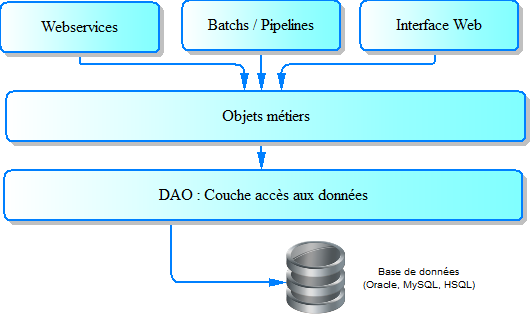
\includegraphics[width=8cm]{images/arch_n_tiers_all.png}
	\end{center}
	\end{frame}

	\begin{frame}
	\frametitle{Architecture n-tiers}
	\framesubtitle{Utilisation Hibernate ORM}
	
	\begin{center}	
	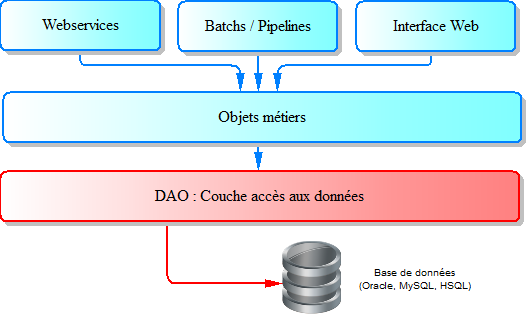
\includegraphics[width=8cm]{images/arch_n_tiers_hibernate.png}
	\end{center}
\end{frame}
	
	
\subsection{Concept Object-relational Mapping}	
		
\begin{frame}{Définition de ORM}
	
	\begin{block}{ORM}
	Mapping objet-relationnel (Object Relational Mapping). Relation entre les objets et les tables.
	\end{block}

	\pause
	\begin{block}{Objectif}	
	Donne l'illusion de travailler avec une base de données \textbf{Orientée Objets}.
	\end{block}
	
\end{frame}
		
\begin{frame}[containsverbatim]{Exemple sans mapping objet-relationnel}
	\framesubtitle{Liste des employés}
	\begin{lstlisting}
	List<Employee> employees = new ArrayList<Employee>();
	Connection conn = getConnection();
	try {
		PreparedStatement ps = conn.prepareStatement("SELECT .. FROM EMPLOYEE WHERE ..." );
		try {
			ResultSet rs = ps.executeQuery();
			try {
				while (rs.next()) {
					Employee employee = new employee();
					employee.setId( rs.getInt(1) );
					employee.setName ( rs.getString(2) );
					// autres parametres ...
					employees.add(employee);
				}
			} finally {
				rs.close();
			}
		} finally{ 
			ps.close(); 
		}
	} catch (SQLException e) { 
		// rollback...
	} finally { 
		conn.close(); 
	}
	
	return list;
	\end{lstlisting}	
	
\end{frame}
	
\begin{frame}
	Problématiques de l'utilisation de JDBC\footnote{couche bas niveau de la persistance SQL en Java} :
	\begin{itemize}
	\item Gestion manuelle de la connexion : dupliquée dans chaque méthode
	\item Mapping \emph{Table / Objets} réalisé manuellement, au moins 1 fois en lecture et 1 fois en écriture
	\item Écriture en SQL natif : nom des champs, dialecte utilisé, \dots
	\end{itemize}
	
	\pause
	\begin{block}{}
	\center
	Et en utilisant un ORM comme \textbf{Hibernate} ?
	\end{block}
		
\end{frame}
		
\begin{frame}[fragile]{Exemple avec Hibernate}
	\framesubtitle{...et Spring}
	
	\begin{itemize}[<+->]
	\item Recherche
	\begin{lstlisting}
List<Employee> employees=session.createQuery("FROM Employees").list();
\end{lstlisting}
	\item Sauvegarde
	\begin{lstlisting}
session.saveOrUpdate(employee);
	\end{lstlisting}	
	\end{itemize}	
\end{frame}

\begin{frame}{Hibernate va plus loin !}
	
	\begin{block}{}
	\center
	Et si l'employé avait des attributs \emph{contrat}, \emph{chef} ?
	\end{block}
	
	\pause
	Ça ne change rien !
	\begin{itemize}
	\item pendant la recherche les attributs sont chargés et accessibles via les \emph{getters}
	\item pendant la sauvegarde, les attributs sont créés ou mis à jour.
	\end{itemize}
	
\end{frame}
	
%%%%%%%%%%%%%%%%%%%%%%%%%%%%%%%%%%%%%%%%%%%%%%
%% Entity Manager
\section{Session (EntityManager)}

\subsection{Le principe}

\begin{frame}{Architecture JDBC}
	
	\begin{center}
	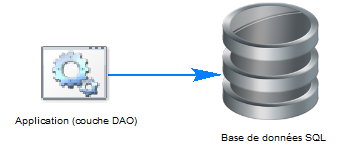
\includegraphics[height=2cm]{images/without_orm.png}	
	\end{center}
	
	\begin{block}{}
	\center
	Tous les traitements métiers sont codés dans l'application.
	\end{block}
\end{frame}
	
\begin{frame}{La session, ou EntityManager}
	\framesubtitle{Unique interface à la base de données !}
	
	\begin{center}
	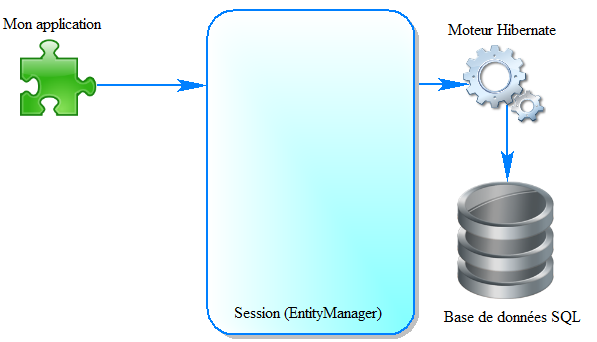
\includegraphics[height=4.5cm]{images/with_orm_empty.png}	
	\end{center}
	
	\begin{block}{}
	\center
	L'application n'a aucune interaction avec la base de données. L'\textbf{unique} point d'entrée est la session.
	\end{block}
\end{frame}

\begin{frame}{Recherche d'objets en BDD}
	\framesubtitle{... mais en passant par la session}
	
	\begin{center}
	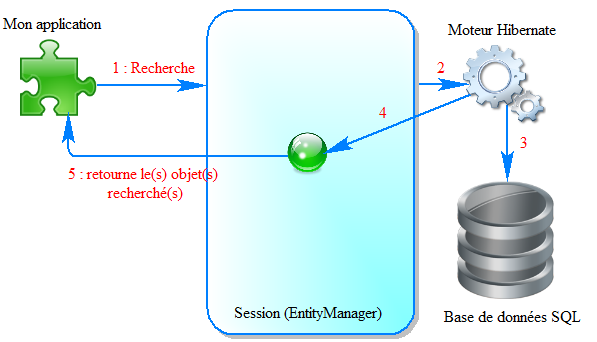
\includegraphics[height=4.5cm]{images/with_orm_select.png}	
	\end{center}
	
	\begin{itemize}
	\item Requête \textbf{objet} sur la \emph{session}
	\item Hibernate traduit la demande et exécute un \texttt{SELECT}
	\item Les objets sont retournés, \textbf{mais restent liés à la session !}
	\end{itemize}
	
	%% ORAL : je ne demande pas les "records" qui sont dans la table Employee et qui ... ; je demande la liste des employés encore actif.
\end{frame}

\begin{frame}{Modification de la session}
	
	\begin{center}
	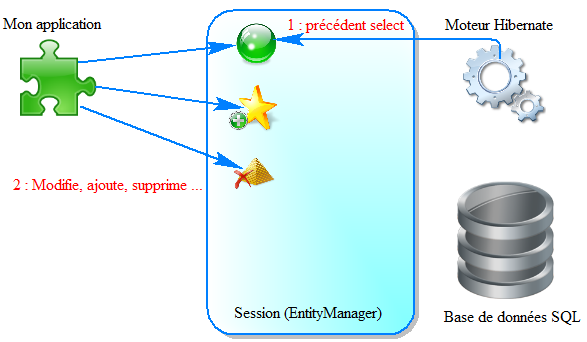
\includegraphics[height=4.5cm]{images/with_orm_modify.png}	
	\end{center}
	
	\begin{itemize}
	\item Modification d'entités déjà liées à la session
	\item Ajout de nouvelle entités à la session
	\item Marquage d'entités comme supprimées
	\end{itemize}
	
	%% ORAL : je ne demande pas les "records" qui sont dans la table Employee et qui ... ; je demande la liste des employés encore actif.
\end{frame}

\begin{frame}{Flush et commit}
	
	\begin{center}
	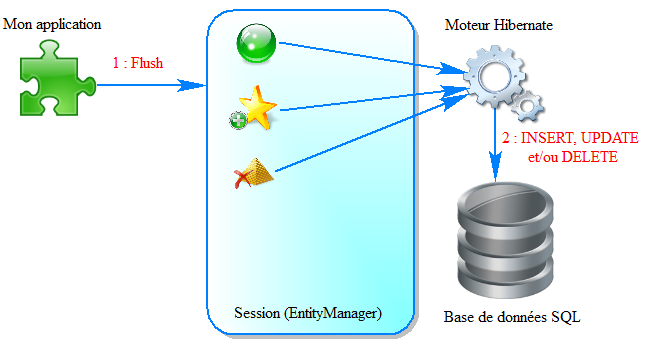
\includegraphics[height=4cm]{images/with_orm_flush.png}	
	\end{center}
	
	\begin{block}{Flush de la Session}
	Tous les entités liés à la session, \emph{et leurs dépendances (attributs)}, sont créés, mis à jour ou supprimés dans la base de données.\\
	\end{block}
	
\end{frame}

\begin{frame}{États des entités}
	
	\begin{center}
	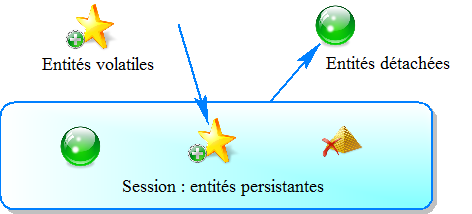
\includegraphics[height=4cm]{images/entities_states.png}	
	\end{center}
	
	\pause
	\begin{itemize}[<+->]
	\item Les nouvelles entités sont dites : \textbf{volatiles} (\texttt{transient})
	\item les entités qui sont liées sont dites : \textbf{persistantes}
	\item les entités dont la session a été fermées sont dites : \textbf{détachées}
	\end{itemize}

\end{frame}


\subsection{Limitations}
\begin{frame}{Limitations de la session}
	\begin{alertblock}{Face aux threads}
	La \emph{session} est un objet \textbf{non-thread-safe}.
	\end{alertblock}

	\pause
	\begin{itemize}
		\item ne pas placer une session en attribut d'un singleton !
	\end{itemize}

	
	\pause
	\begin{block}{Bonne pratique}
	1 session = 1 transaction.
	\end{block}
	
\end{frame}



\subsection{La SessionFactory}

\begin{frame}{La \emph{SessionFatory}}
	\framesubtitle{Usine de sessions}
	
	\begin{block}{SessionFatory}
	La \emph{SessionFatory} est une fabrique de \emph{sessions}. Elle n'est créée qu'une seule fois, au lancement de l'application.
	\end{block}	
	
	\pause	
	Configration dans \texttt{hibernate.hbm.xml} :
	\begin{itemize}
	\item Source de données (fabrique de connexions à la BDD)
	\item Mapping objet : relation entre les tables et les objets
	\item Politiques de chargement, cache, ... tout ou presque est surchargeable !
	\end{itemize}
\end{frame}

	
\subsection{Un peu de code ...}

\begin{frame}[containsverbatim]{Un peu de code ...}
	\framesubtitle{... sans l'aide de Spring}
	
	\begin{itemize}
	\item Recherche uniquement (read only) : 	
	\end{itemize}	
	\begin{lstlisting}
	// Obtention d'une session
	Session session = sessionFactory.openSession();
	
	// MON CODE ICI	
	
	// Fermeture de la session
	session.close();
	\end{lstlisting}
	
\end{frame}

\begin{frame}[containsverbatim]{Un peu de code ...}
	\framesubtitle{... sans l'aide de Spring}
	
	\begin{itemize}
	\item Modification (read-write) :
	\end{itemize}	
	\begin{lstlisting}
	// Obtention d'une session
	Session session = sessionFactory.openSession();
 
 	// Debut de la transaction
	session.beginTransaction();
	try {
		// MON CODE ICI	
	
		// Commit de la session si c'est OK
		session.getTransaction().commit();
		
	} catch (Exception e) {
		// On annule tout ce qui a ete fait si une erreur s'est produite
		session.getTransaction().rollback();
		throw e;
		
	} finally {
		session.close();
	}
	\end{lstlisting}
	
\end{frame}


\begin{frame}{Sauvegarde d'une entité}
 	
 	\begin{block}{Sauvegarder ou mettre à jour}
	Pour sauvegarder un objet, il faut le lier à la session. Il sera inséré en BDD lors du commit de la transaction (flush).
	\end{block}
	
	\pause
	\begin{alertblock}{1 seule entité par enregistrement}
	Il ne peut pas y avoir 2 instances d'une même classe avec la même clé primaire.
	\end{alertblock}
	
\end{frame}

\begin{frame}[fragile]{Sauvegarde d'une entité}
 	\framesubtitle{Save, persist, update, merge, ... ?}
 	
	Plusieurs cas sont possibles :
	\begin{itemize}[<+->]
	\item \texttt{saveOrUpdate} : pour toute entité, quelque soit sont état
	\item \texttt{save} : nouvelle entité (et enregistrement en base), pas d'identifiant
	\item \texttt{update} : entité existant déjà en base, avec son identifiant renseigné 
	\item \texttt{persit} : exécute immédiatement l'insertion (pas/peu de vérification d'existence) 
	\item \texttt{merge} : remplace l'instance de même id déjà liée à la session
	\end{itemize}
	
	\begin{lstlisting}
	// Ajout d'une entite a la session
	session.saveOrUpdate(myEntity);
	\end{lstlisting}
	
\end{frame}

\begin{frame}[fragile]{Supprimer une entité}
	
	\begin{lstlisting}
	// Supprime l'entite
	session.delete(myEntity);
	\end{lstlisting}
\end{frame}


\begin{frame}[fragile]{Charger une entité}
	Rechercher une entité par son identifiant base de données :
	\begin{lstlisting}
	// Charche une entite a partir d'un identifiant (serialisable)
	session.get(Employee.class, id);
	\end{lstlisting}
\end{frame}
	
\subsection{Résumé sur l'utilisation des sessions}

\begin{frame}{Utilisation d'une session}
	\framesubtitle{Rappels...}
	
	\begin{block}{Sauvegarde des entités}
	Pour être sauvegardée, une entité doit être \textbf{persistante} : liée à la session.
	\end{block}
	
	\pause
	\begin{block}{Rendre persistante une entité}
	Une entité est rendu persistante lors de l'appel des méthodes de la session : \texttt{saveOrUpdate} ou \texttt{delete}.
	\end{block}
	
	\pause
	\begin{block}{Entités recherchées}
	Les entités retournées par la session suite à une recherche sont déjà persistantes.
	\end{block}	
\end{frame}
	
%%%%%%%%%%%%%%%%%%%%%%%%%%%%%%%%%%%%%%%%%%%%%
%% Mapping à proprement parlé
\section{Relation objets / tables}

\subsection{Modèle d'exemple}

\begin{frame}{Modèle entreprise et employés}
	\begin{center}
	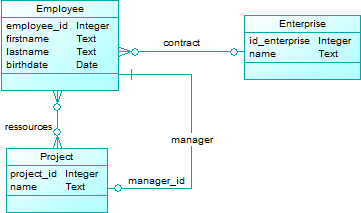
\includegraphics{images/model_employees_full.png}	
	\end{center}
\end{frame}

\subsection{Configuration de mapping minimale}
\begin{frame}{Déclaration d'une entité}
	\framesubtitle{Annotations obligatoires}
	
	Seules 2 annotations sont obligatoires pour déclarer qu'une \textbf{classe est persistante} :
	\pause
	\begin{itemize}[<+->]
		\item \texttt{$@$Entity} : indique a Hibernate que la classe est persistante
		\item \texttt{$@$Id} : les entités doivent obligatoirement avoir un ID
	\end{itemize}
	
\end{frame}

\begin{frame}[fragile]{Déclaration d'une entité}
	\framesubtitle{Configuration de mapping minimale}
	
	\begin{lstlisting}
	@Entity
	public class Employee implements Serializable {
	  private Integer id;
	  
	  @Id
	  public Integer getId() {
	    return id;
	  }
	  
	  public void setId(Integer id) {
	    this.id = id;
	  }
	}
	\end{lstlisting}
	
	\pause
	Equivalance BDD : 
	\begin{lstlisting}
	CREATE TABLE employee (
	  id INTEGER PRIMARY KEY
	);
	\end{lstlisting}
	
\end{frame}

\begin{frame}{Mapping des autres attributs/champs}

	\begin{block}{Nommage des champs}
		Par défaut, le nom des champs et tables de la BDD sont ceux des attributs et classes.
	\end{block}

	\pause
	\begin{block}{Déclaration d'autres attributs}
		Les méthodes commençant par \texttt{get} seront considérées comme des attributs persistant. L'annotation \texttt{$@$Transient} annule cette définition.
	\end{block}
	
\end{frame}


\subsection{Personalisations des noms}
\begin{frame}[fragile]{Personalisations des noms}
	
	\begin{lstlisting}
@Entity
@Table(name = "employees_table")
public class Employee implements Serializable {

  @Id
  @GeneratedValue(strategy=GenerationType.IDENTITY)
  @Column(name = "employee_id")
  public Integer getId() {...}
    
  @Column(name = "name")
  public String getLastname() { ... }
  
  public Date getBirthdate() { ... }
}
	\end{lstlisting}
	
	\pause
	Equivalance BDD : 
	\begin{lstlisting}
CREATE TABLE employees_table (
  employee_id INTEGER NOT NULL AUTO_INCREMENT,
  name VARCHAR(255),
  birthdate DATE,
  
  PRIMARY KEY (employee_id)
);
	\end{lstlisting}
	
\end{frame}


\subsection{Relations}

\begin{frame}{Définition des relations}
	\framesubtitle{Les 3 types de relations pricipales}
	
	Exemple des associations les plus communes :
	\begin{itemize}[<+->]
		\item OneToOne : relation entre une personne et son passeport
		\item OneToMany et ManyToOne : Relations entre un régiment et des soldats
		\item ManyToMany : relations entre les magasins et les clients
	\end{itemize}

\end{frame}


\begin{frame}[fragile]{Relations OneToMany -- ManyToOne}
	\framesubtitle{Un employé et son entreprise}
	
	\begin{itemize}
		\item Classe \texttt{Employee} : 
		\begin{lstlisting}
// 'enterprise_id' est le nom de la colonne clef etrangere presente dans la table employee.
@ManyToOne(cascade=CascadeType.ALL)
@JoinColumn(name = "enterprise_id")
public Enterprise getEnterprise() { ... }
		\end{lstlisting}
	
		\item Classe \texttt{Enterprise}
		\begin{lstlisting}
// 'enterprise' est le nom de l'attribut dans la classe Employee
@OneToMany(mappedBy = "enterprise", cascade=CascadeType.ALL)
public Set<Employee> getEmployees() { ... }
		\end{lstlisting}	
	\end{itemize}

\end{frame}

\begin{frame}[fragile]{Relations ManyToMany}
	\framesubtitle{Des employés et des projets}
	
	\begin{itemize}
		\item Classe \texttt{Employee} : 
		\begin{lstlisting}
// 'EMPLOYEE_PROJECT' est le nom de la table de jointure
// EMPLOYEE_ID est le nom de la clef etrangere table de jointure -> table EMPLOYEE
// PROJECT_ID est le nom de la clef etrangere table de jointure -> table PROJECT
@ManyToMany(cascade = CascadeType.ALL)
@JoinTable(
	name="EMPLOYEE_PROJECT",
	joinColumns=@JoinColumn(name="EMPLOYEE_ID"),
	inverseJoinColumns=@JoinColumn(name="PROJECT_ID")
)
public Set<Project> getProjects() { ... }
		\end{lstlisting}
	
		\item Classe \texttt{Project}
		\begin{lstlisting}
// 'projects' est le nom de l'attribut dans la classe Employee
@ManyToMany(
	cascade = CascadeType.ALL,
	mappedBy = "projects"
)
public Set<Employee> getEmployees() { ... }
		\end{lstlisting}	
	\end{itemize}

\end{frame}


%% Contraintes ?

	
%%%%%%%%%%%%%%%%%%%%%%%%%%%%%%%%%%%%%%%%%%%%%
%% Requêtes sur la base
\section{Requêtes de recherches}

\begin{frame}{Les différents langages de requêtage}
	2 façons d'exécuter une requête de recherche :
	\begin{itemize}[<+->]
		\item \textbf{HQL} : dérivé du langage SQL, se présente comme une chaine de caractères. Permet aussi les UPDATE et DELETE.
		\item \textbf{L'API Criteria} : d'écriture des requêtes sous forme d'objets
	\end{itemize}

\end{frame}


\subsection{Langage HQL}

\begin{frame}[fragile]{Le langage HQL}
	\framesubtitle{Ecriture d'une requête}
	
	Une requête s'écrit : 
	\begin{lstlisting}
Query query = session.createQuery(myRequest);
query.setParameter("prenom", "HisFirstName");
query.setParameter("nom", "HisLastName");

List<Employee> employees = query.list();
	\end{lstlisting}

\end{frame}

\begin{frame}[fragile]{Le langage HQL}
	\framesubtitle{Les basics}
	
	\begin{block}{}
		\center
		Lister le contenu de la table \texttt{employee}
	\end{block}
	
	\begin{exampleblock}{SQL}
		\texttt{SELECT * FROM employee;}
	\end{exampleblock}

	\pause
	\begin{exampleblock}{HQL}
		\texttt{FROM Employee}
	\end{exampleblock}
	
	\pause
	\begin{itemize}
		\item Le terme \texttt{SELECT} est facultatif. Cette notation équivaut à "\texttt{SELECT e FROM Employee e}".
		\item La valeur de la clause \texttt{FROM} est \textbf{le nom de la classe} (pas de la table).
	\end{itemize}

\end{frame}

\begin{frame}[fragile]{Le langage HQL}
	\framesubtitle{Les conditions}
	
	\begin{block}{}
		\center
		Rechercher des employés par leur nom et leur prénom
	\end{block}
	
	\begin{exampleblock}{SQL}
		\texttt{SELECT * FROM employee WHERE lastname = ? AND firstname = ?;}
	\end{exampleblock}

	\pause
	\begin{exampleblock}{HQL}
		\texttt{FROM Employee WHERE lastname = :nom AND firstname = :prenom}
	\end{exampleblock}

\end{frame}


\begin{frame}[fragile]{Le langage HQL}
	\framesubtitle{Les conditions avec des associations *ToOne}
	
	\begin{block}{}
		\center
		Rechercher les employés qui travaillent dans une entreprise (retrouvée par son nom).
	\end{block}
	
	\begin{exampleblock}{SQL}
	\begin{lstlisting}
SELECT emp.*
FROM employee emp
    INNER JOIN enterprise ent ON emp.enterprise_id = ent.enterprise_id
WHERE ent.name = ?;
	\end{lstlisting}
	\end{exampleblock}

	\pause
	\begin{exampleblock}{HQL}
		\texttt{FROM Employee WHERE enterprise.name = :enterpriseName}
	\end{exampleblock}

\end{frame}

\begin{frame}[fragile]{Le langage HQL}
	\framesubtitle{Les conditions avec des associations *ToMany}
	
	\begin{block}{}
		\center
		Rechercher des employés qui travaillent pour un chef de projets.
	\end{block}
	
	\begin{exampleblock}{SQL}
	\begin{lstlisting}
SELECT DISTINCT e.*
FROM employee e
    INNER JOIN employee_project ON e.employee_id = ep.employee_id
    INNER JOIN project ON ep.project_id = p.projet_id
WHERE p.manager_id = ?;
	\end{lstlisting}
	\end{exampleblock}
	
	\pause
	\begin{exampleblock}{HQL (plusieurs solutions ...)}
	\begin{lstlisting}
SELECT DISTINCT p.employees FROM Project p WHERE manager = :manager
	\end{lstlisting}
	\pause
	\begin{lstlisting}
SELECT DISTINCT e
FROM Employee e INNER JOIN e.projects p
WHERE p.manager = :manager
	\end{lstlisting}
	\end{exampleblock}

\end{frame}


\subsection{Langage Criteria}

\begin{frame}[fragile]{L'API Criteria}
	\framesubtitle{L'alternative au HQL...}

	\begin{block}{Criteria}
		Écriture de la requête sous la forme d'un objet JAVA.
	\end{block}		
	
	\pause
	Recherche des employés par leur nom et leur prénom :
	\begin{lstlisting}
// SELECT * FROM employee WHERE lastname = ? AND firstname = ?;
Criteria criteria = session.createCriteria(Employee.class);
criteria.add(Restrictions.eq("lastname", "HisLastName");
criteria.add(Restrictions.eq("firstname", "HisFirstName");

List<Employee> employees = criteria.list();
	\end{lstlisting}

\end{frame}
	
	
	
%%%%%%%%%%%%%%%%%%%%%%%%%%%%%%%%%%%%%%%%%%%%%
%% FIN 
\section{Conclusion}

\subsection{Résumé}
\begin{frame}{Résumé}
	\framesubtitle{Hibernate c'est trop bien !}
	Les points les plus importants :
	\begin{itemize}[<+->]
		\item pour déclarer une  \emph{classe persistante}, les annotations obligatoires sont : \texttt{$@$Entity} et \texttt{$@$Id}
		\item accesseurs (getters et setters) obligatoires
		\item seules les entités liées à la session seront sauvegardées, updatées ou supprimées
		\item pour lier une entité à la session : \texttt{saveOrUpdate} ou \texttt{delete}
	\end{itemize}
\end{frame}
	
\subsection{Fin}
\begin{frame}
	\frametitle{Fin}
	\begin{center}
		\huge
		Merci, des questions ?
	\end{center}
\end{frame}

\end{document}
